\documentclass{beamer}
\usepackage[utf8]{inputenc}
\usepackage[french]{babel}
\usepackage{graphicx}
\usepackage{amsmath}
\usepackage{amssymb}
\usepackage{hyperref}
\usepackage{eso-pic}
\usepackage{listings}
\usepackage[export]{adjustbox}
\usepackage{multicol}
\usepackage[font=small,labelfont=bf]{caption}
\usepackage{xcolor}
\usepackage[linesnumbered,ruled,french,onelanguage]{algorithm 2e}
\usepackage{tikz}
\usepackage{natbib}
\usetikzlibrary{shapes,arrows}
\usetheme{Madrid}

\makeatletter
\g@addto@macro {\@algocf@init}{\SetKwInput{KwOut}{ Sortie}}
\makeatother

\title{ANALYSEUR DE LIVRE DONT VOUS ETES LE HERO (LDVELH)}
\author{KAMGANG KENMOE Miguel Jordan \newline SISSOKO Dioukou Moussa
\newline ABOGOUNRIN Ayath \newline ALHAZZAA Laith  }
\institute{UE : Conception logicielle 1
\newline \newline Université de Caen Normandie }


\definecolor{codeblue}{rgb}{0,0,255}
\definecolor{codegreen}{rgb}{0,0.6,0}
\definecolor{codered}{rgb}{255,0,0}

\lstdefinestyle{mystyle}{
keywordstyle=\color{codeblue},
commentstyle=\color{codegreen},
stringstyle=\color{codered},
title=\lstname
}

\lstset{style=mystyle}

\begin{document}

\begin{frame}
\titlepage

\end{frame}

\begin{frame}
\frametitle{Sommaire}
\tableofcontents
\end{frame}

\section{• Introduction}

\begin{frame}
\frametitle{Introduction}
\framesubtitle {Choix du projet}

\begin{itemize}
\item Notre intérêt pour les livres dont vous êtes le héro.
\item Apprendre la notion des graphes.
\end{itemize}
\end{frame}

\begin{frame}
\frametitle{Introduction}

\begin{columns}
\begin{column}{0.5\textwidth}

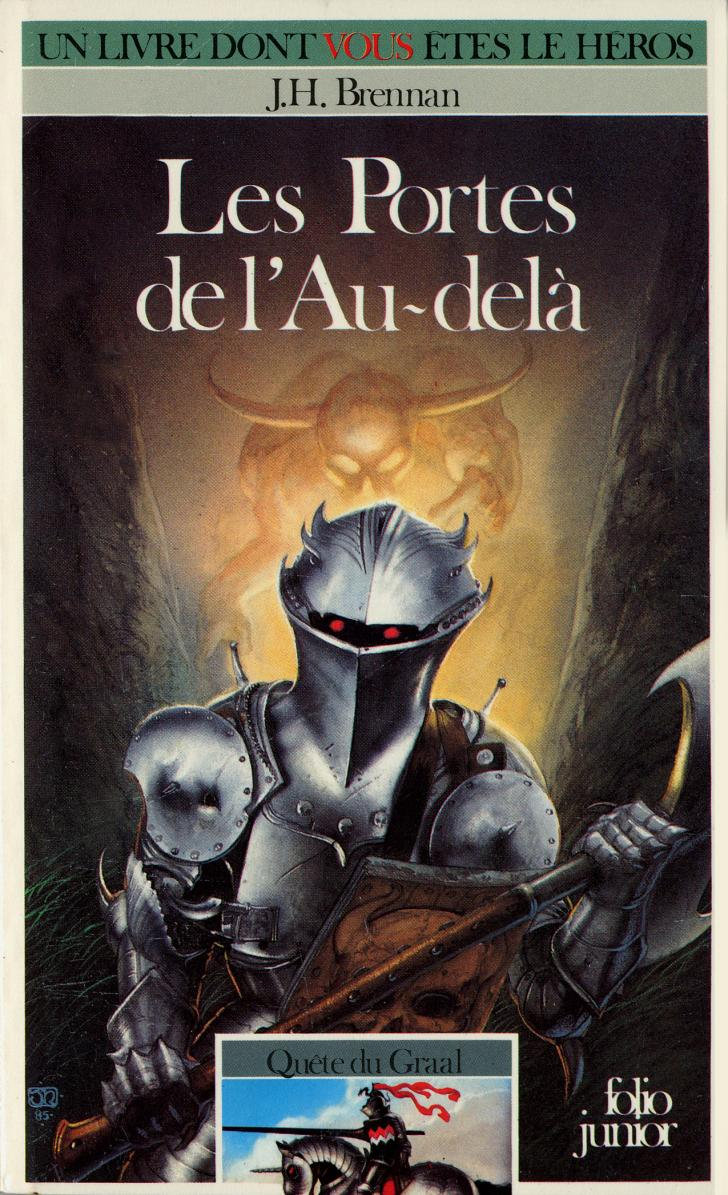
\includegraphics[width=\textwidth ,height=7.5cm]{images/livre.jpg}
\end{column}

\begin{column}{0.5\textwidth}
\begin{itemize}
\item C'est quoi un livre dont vous etes le héro ?
\item C'est quoi un analyseur de livre ?
\end{itemize}
\end{column}
\end{columns}
\end{frame}

\begin{frame}
\section{• Objectifs du projet}
\frametitle{Objectifs du projet}
\framesubtitle {Description détaillée}
 
 \begin{itemize}
 \item Obtenir un graphe à partir d'un fichier JSON ou d'un fichier TXT.
 \item Afficher un graphe à l'aide d'un algorithme de force.
 \item Implémenter différents algorithmes pour analyser le graphe.
 \item Étendre le modèle du graphe.
\end{itemize}
\end{frame}

\begin{frame}
\section{• Fonctionnalités implémentées}
\frametitle{Fonctionnalités implémentées}
\framesubtitle {Descriptions des fonctionnalités}
\begin{center}
    	\begin{tikzpicture}
    		\node (ex)[rectangle, draw = blue, blue, fill = yellow] at (-5,2) {extraction};
    		\node (m)[rectangle, draw = blue, blue, fill = yellow] at (3,2) {model};
    		\node (b)[rectangle, draw = blue, blue, fill = yellow] at (-1,4) {backbone};
    		
    		
        	\node (bl)[rectangle, draw = black] at (-1.2,1) {BookLabel};
        	\node (jb)[rectangle, draw = black] at (-3.4, 1) {JsonBuilder};
        	\node (tb)[rectangle, draw = black] at (-5.6, 1) {TextBuilder};
        	
        	\node (bo)[rectangle, draw = white, white , fill = blue] at (0, 2) {Book};
        	\node (p)[rectangle, draw = black] at (-1.5, 2) {Page};
        	
        	\node (n)[rectangle, draw = black] at (1, 1) {Node};
        	\node (e)[rectangle, draw = black] at (3, 1) {Edge};
        	\node (g)[rectangle, draw = black] at (5, 1) {Graph};
        	
        	\draw[->] (b.210) -- (bo.510);
        	\draw[->] (b.210) -- (p.510);
        	
        	\draw[->] (ex.210) -- (bl.510);
        	\draw[->] (ex.210) -- (jb.510);
        	\draw[->] (ex.210) -- (tb.510);
        	
        	\draw[->] (m.210) -- (n.510);
        	\draw[->] (m.210) -- (e.510);
        	\draw[->] (m.210) -- (g.510);
        	
        	\draw[->] (ex.510) -- (b.210);
        	\draw[->] (m.510) -- (b.210);
    	\end{tikzpicture}
    \end{center}
\end{frame}

\begin{frame}
	\frametitle{Fonctionnalités implémentées}
	\framesubtitle{Description des paquetages}
	\begin{minipage}[t]{0.5\linewidth}
		\begin{enumerate}
			\item Racine
			\item Système MVC
			\item Notre graphe est fixe et l'inutilité de controller 
			\item Le changement et son utilité pour notre graphe 
		\end{enumerate}
	\end{minipage}
	\begin{minipage}[t]{0.35\linewidth}
		\begin{flushright}
			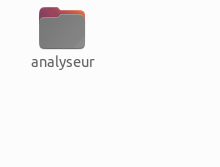
\includegraphics[width =\linewidth]{images/image.png}
			\vspace{1em}
			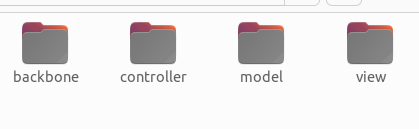
\includegraphics[width =\linewidth]{images/image3.png}
			\vspace{1em}			
			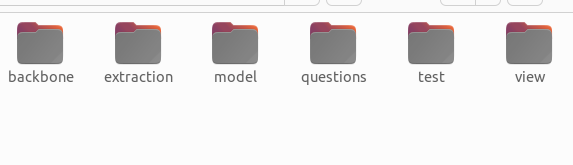
\includegraphics[width =\linewidth]{images/image2.png}
			\vspace{1em}
		\end{flushright}
	\end{minipage}
\end{frame}

\begin{frame}
\section{• Éléments techniques}
\frametitle{Éléments techniques}
\framesubtitle {Répartition des tâches}
	\begin{center}
    	\begin{tikzpicture}
    		\node (mi)[rectangle, draw = blue, blue, fill = yellow] at (1,4) {Miguel};
    		\node (a)[rectangle, draw = blue, blue, fill = yellow] at (-1,4) {Ayath};
    		\node (l)[rectangle, draw = blue, blue, fill = yellow] at (5,4) {Laith};
    		\node (mo)[rectangle, draw = blue, blue, fill = yellow] at (3,4) {Moussa};
    		
        	\node (e)[rectangle, draw = black] at (-1,1) {extraction};
        	\node (v)[rectangle, draw = black] at (1, 1) {view};
        	\node (m)[rectangle, draw = black] at (3, 1) {model};
        	\node (q)[rectangle, draw = black] at (7, 1) {questions};
        	\node (t)[rectangle, draw = black] at (5, 1) {test};
        	\node (b)[rectangle, draw = black] at (-3, 1) {backbone};
        	\node (p)[rectangle, draw = blue, blue] at (2.5, -1){ANALYSEUR DE LIVRE DONT VOUS 						ETES LE HERO};
        	\draw[->] (mi.210) -- (e.510);
        	\draw[->] (a.210) -- (v.510);
        	\draw[->] (mi.210) -- (v.510);
        	\draw[->] (l.210) -- (q.510);
        	\draw[->] (mo.210) -- (q.510);
        	\draw[->] (mi.210) -- (m.510);
        	\draw[->] (mo.210) -- (m.510);
        	\draw[->] (e.210) -- (p.510);
        	\draw[->] (m.210) -- (p.510);
        	\draw[->] (t.210) -- (p.510);
        	\draw[->] (v.210) -- (p.510);
        	\draw[->] (q.210) -- (p.510);
        	\draw[->] (b.210) -- (p.510);
        	\draw[->] (mo.210) -- (t.510);
        	\draw[->] (a.210) -- (m.510);
        	\draw[->] (l.210) -- (m.510);
        	\draw[->] (mi.210) -- (b.510);
        	\draw[->] (mo.210) -- (b.510);
        	\draw[->] (a.210) -- (b.510);
        	\draw[->] (l.210) -- (b.510);
        	
    	\end{tikzpicture}
    \end{center}
\end{frame}

\begin{frame}
\frametitle{Éléments techniques}
\framesubtitle{Descriptions des algorithmes}

Dans ce projet nous avons exploré plusieurs algorithmes tels que : 

\begin{itemize}
\item Fruchterman Reingold
\item Kamada-Kawai
\item Dijkstra
\item Breath First Search
\item Depth First Search Directed Acyclic Graphs
\item Tri topologique
\end{itemize}
\end{frame}

\begin{frame}[fragile]
\frametitle{Éléments techniques}
\framesubtitle{Pseudocode de l'algorithme de Fruchterman-Reingold (Partie 1)}

\begin{algorithm}[H]
\DontPrintSemicolon
\small
\small
\small
\SetAlgoLined
\SetKwFunction{fa}{fa}
\SetKwFunction{fr}{fr}
\SetKwFunction{cool}{cool}

\SetKwInOut{Input}{Entrées}
\SetKwInOut{Output}{Sorties}

\Input{Largeur $W$, Longueur $L$, Ensemble de Sommets $V$, Ensemble d'Arêtes $E$, Nombre d'itérations}
\Output{Positions finales des sommets}

$area \gets W \times L$\;
$G \gets (V, E)$\;
$k \gets \sqrt{\frac{area}{|V|}}$\;

\SetKwFunction{disp}{disp}

\For{$i \gets 1$ \KwTo iterations}{
    \For{$v$ \textbf{in} $V$}{
        $v.\disp \gets (0,0)$\;
        \For{$u$ \textbf{in} $V$}{
            \If{$u \neq v$}{
                $\delta \gets v.\text{pos} - u.\text{pos}$\;
                $v.\disp \gets v.\disp + \frac{\delta}{|\delta|} \times \fr(|\delta|)$\;
            }
        }
    }}
\end{algorithm}

\end{frame}

\begin{frame}[fragile]
\frametitle{Éléments techniques}
\framesubtitle{Pseudocode de l'algorithme de Fruchterman-Reingold (Partie 2)}

\begin{algorithm}[H]
\DontPrintSemicolon
\small
\SetAlgoLined
\SetKwFunction{fa}{fa}
\SetKwFunction{fr}{fr}
\SetKwFunction{cool}{cool}

\SetKwInOut{Input}{Entrées}
\SetKwInOut{Output}{Sorties}

\Input{Largeur $W$, Longueur $L$, Ensemble de Sommets $V$, Ensemble d'Arêtes $E$, Nombre d'itérations}
\Output{Positions finales des sommets}

\For{$e$ \textbf{in} $E$}{
    $\delta \gets e.v.\text{pos} - e.u.\text{pos}$\;
    $e.v.\disp \gets e.v.\disp - \frac{\delta}{|\delta|} \times \fa(|\delta|)$\;
    $e.u.\disp \gets e.u.\disp + \frac{\delta}{|\delta|} \times \fa(|\delta|)$\;
}
\end{algorithm}

\end{frame}

\begin{frame}[fragile]
\frametitle{Éléments techniques}
\framesubtitle{Pseudocode de l'algorithme de Fruchterman-Reingold (Partie 3)}

\begin{algorithm}[H]
\DontPrintSemicolon
\small
\SetAlgoLined
\SetKwFunction{fa}{fa}
\SetKwFunction{fr}{fr}
\SetKwFunction{cool}{cool}

\SetKwInOut{Input}{Entrées}
\SetKwInOut{Output}{Sorties}

\Input{Largeur $W$, Longueur $L$, Ensemble de Sommets $V$, Ensemble d'Arêtes $E$, Nombre d'itérations}
\Output{Positions finales des sommets}

\For{$v$ \textbf{in} $V$}{
    $v.\text{pos} \gets v.\text{pos} + \frac{v.\disp}{|v.\disp|} \times \min(v.\disp, t)$\;
    $v.\text{pos.x} \gets \min(\frac{W}{2}, \max(-\frac{W}{2}, v.\text{pos.x}))$\;
    $v.\text{pos.y} \gets \min(\frac{L}{2}, \max(-\frac{L}{2}, v.\text{pos.y}))$\;
}
$t \gets \text{cool}(t)$\;

\end{algorithm}

\end{frame}

\begin{frame}
\frametitle{Éléments techniques}
\framesubtitle{Affichage du graphe sans le facteur de refroidissement}

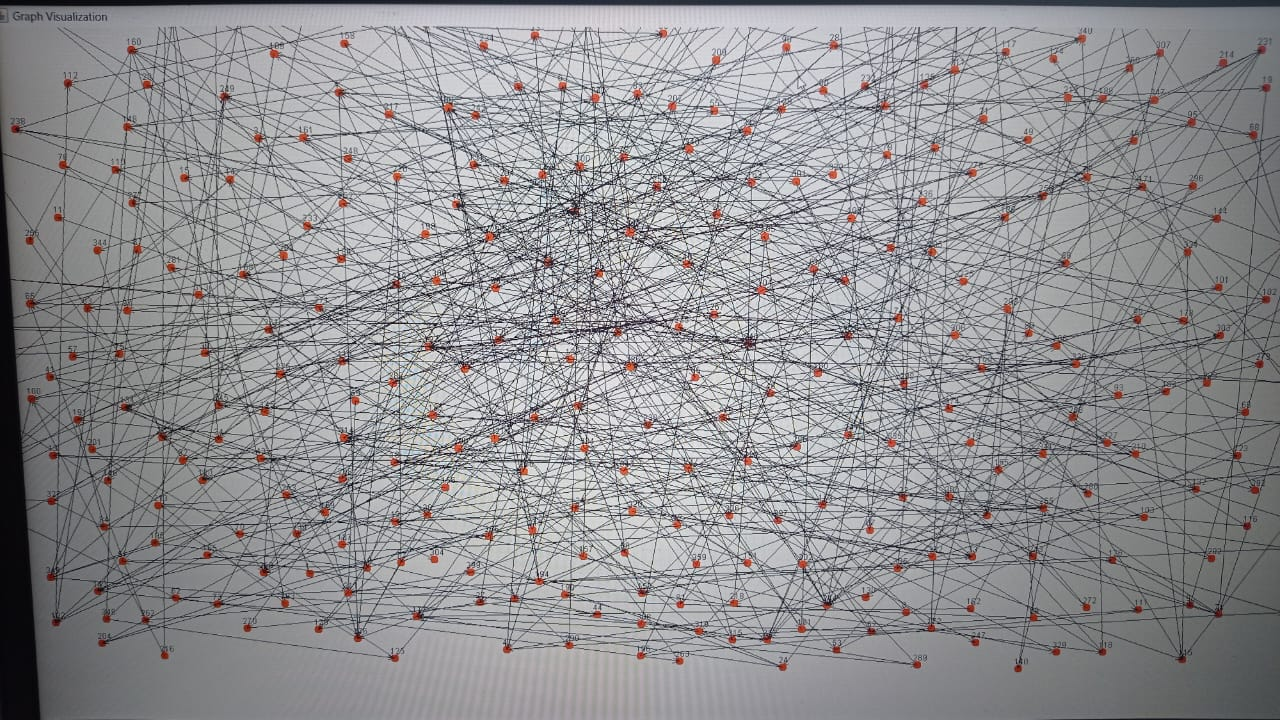
\includegraphics[width=\textwidth ,height=7cm]{images/ancienGraphe.jpeg}
\end{frame}



\begin{frame}
\frametitle{Expérimentations et usages}
\framesubtitle {Résultats quantifiables}

A présent montrons à quoi resemble le projet une fois executé, à savoir que son exécution est divisée en trois :
\begin{itemize}
    \item Affichage du graphe dans une interface graphique : java -jar Graph.jar
    \item Affichage dans la console des éléments d'analyse du graphe :java -jar Analyse.jar
    \item Affichage du résultat des Tests effectués sur le graphe : java -jar Test.jar
\end{itemize}
\end{frame}

\begin{frame}
\section{• Conclusion}
\frametitle{Conclusion}
\framesubtitle{Récapitulatif des fonctionnalités principales}
\centering
Récapitulatif 
\end{frame}

\begin{frame}
\frametitle{Conclusion}
\framesubtitle{Propositions d’améliorations}
\begin{itemize}
 \item Implémentation de l'algorithme de Dijkstra afin de voir la plus rapide parmi les deux et d'opter pour ça.
 \item Revoir l'affichage de notre graphe pour avoir le même graphe à chaque fois qu'on lance le main,ne plus avoir des dispositions aléatoire des nœuds.
 \item Ajouter les inventaires.                                             

\end{itemize}
\end{frame}
\end{document}
